%%%%%%%%%%%%%%%%%%%%%%%%%%%%%%%%%%%%%%%%%
% Memo
% LaTeX Template
% Version 1.0 (30/12/13)
%
% This template has been downloaded from:
% http://www.LaTeXTemplates.com
%
% Original author:
% Rob Oakes (http://www.oak-tree.us) with modifications by:
% Vel (vel@latextemplates.com)
%
% License:
% CC BY-NC-SA 3.0 (http://creativecommons.org/licenses/by-nc-sa/3.0/)
%
%%%%%%%%%%%%%%%%%%%%%%%%%%%%%%%%%%%%%%%%%

\documentclass[letterpaper,11pt]{texMemo} % Set the paper size (letterpaper, a4paper, etc) and font size (10pt, 11pt or 12pt)

\usepackage{parskip} % Adds spacing between paragraphs
\usepackage[colorlinks]{hyperref}
\usepackage{graphicx}
\usepackage{float}
\usepackage{hyperref}
\usepackage{listings}
\hypersetup{citecolor=DeepPink4}
\hypersetup{linkcolor=red}
\hypersetup{urlcolor=blue}
\usepackage{cleveref}
\setlength{\parindent}{15pt} % Indent paragraphs

%----------------------------------------------------------------------------------------
%	MEMO INFORMATION
%----------------------------------------------------------------------------------------

\memoto{Dr.Randy Hoover} % Recipient(s)

\memofrom{Benjamin LeBrun, Benjamin Garcia} % Sender(s)

\memosubject{Lab Assignment 7: TC2 and Servo Control } % Memo subject

\memodate{\today} % Date, set to \today for automatically printing todays date

% \logo{\includegraphics[width=0.1\textwidth]{logo.png}} % Institution logo at the top right of the memo, comment out this line for no logo

%----------------------------------------------------------------------------------------

\begin{document}

\maketitle % Print the memo header information

%----------------------------------------------------------------------------------------
%	MEMO CONTENT
%----------------------------------------------------------------------------------------

\section*{Introduction}
For this lab, we utilized second internal timer to the Atmega328p to produce a PWM signal
to drive our robot car's servo. This required activating Timer 2 on control pin 3 and 
correctly setting it to output a 50 Hz control signal. This will be used to move the 
ultrasonic sensor 90 degrees left and right of our robot to effectively maneuvere around 
obsticles and walls.

\section*{Equipment}
The primary devices we used were:

\begin{itemize}
    \item Acrylic vehicle body with screws, assembled
    \item Elegoo Uno (chip: Atmega328p)
    \item HC-SR04 ultrasonic distance sensor
    \item SG 90 hobby servo motor
    \item 2 ICR18650 batteries with battery box
    \item Ribbon cables
    \item Host laptop with AVR-gcc 8-bit toolchain
    \item USB 2.0 A to B cable
\end{itemize}

\subsection*{Configuration}
Our robot vehicle was assembled according to Elegoo's instructions which can be found
on Elegoo's website at \url{https://www.elegoo.com/download/}. For this lab, we are
using the V3.0 version of the robot kit.

While the timers and configuration are similar to the configuration and driving of the 
DC motors using PWM modes from the Arduino's built in timers, for our servo we require a 
different operating frequency than our DC motor needs. In our case, we needed to generate 
a 50 Hz PWM signal from the second Timer, which required using Phase corrected mode instead 
of the DC motor's fast PWM mode and then writing a correct pulse width to the count registers.

This allows us to call a single function with the degree angle between 0 and 180 degrees with 0
being the leftmost position.

\begin{figure}[!ht]
\begin{center}
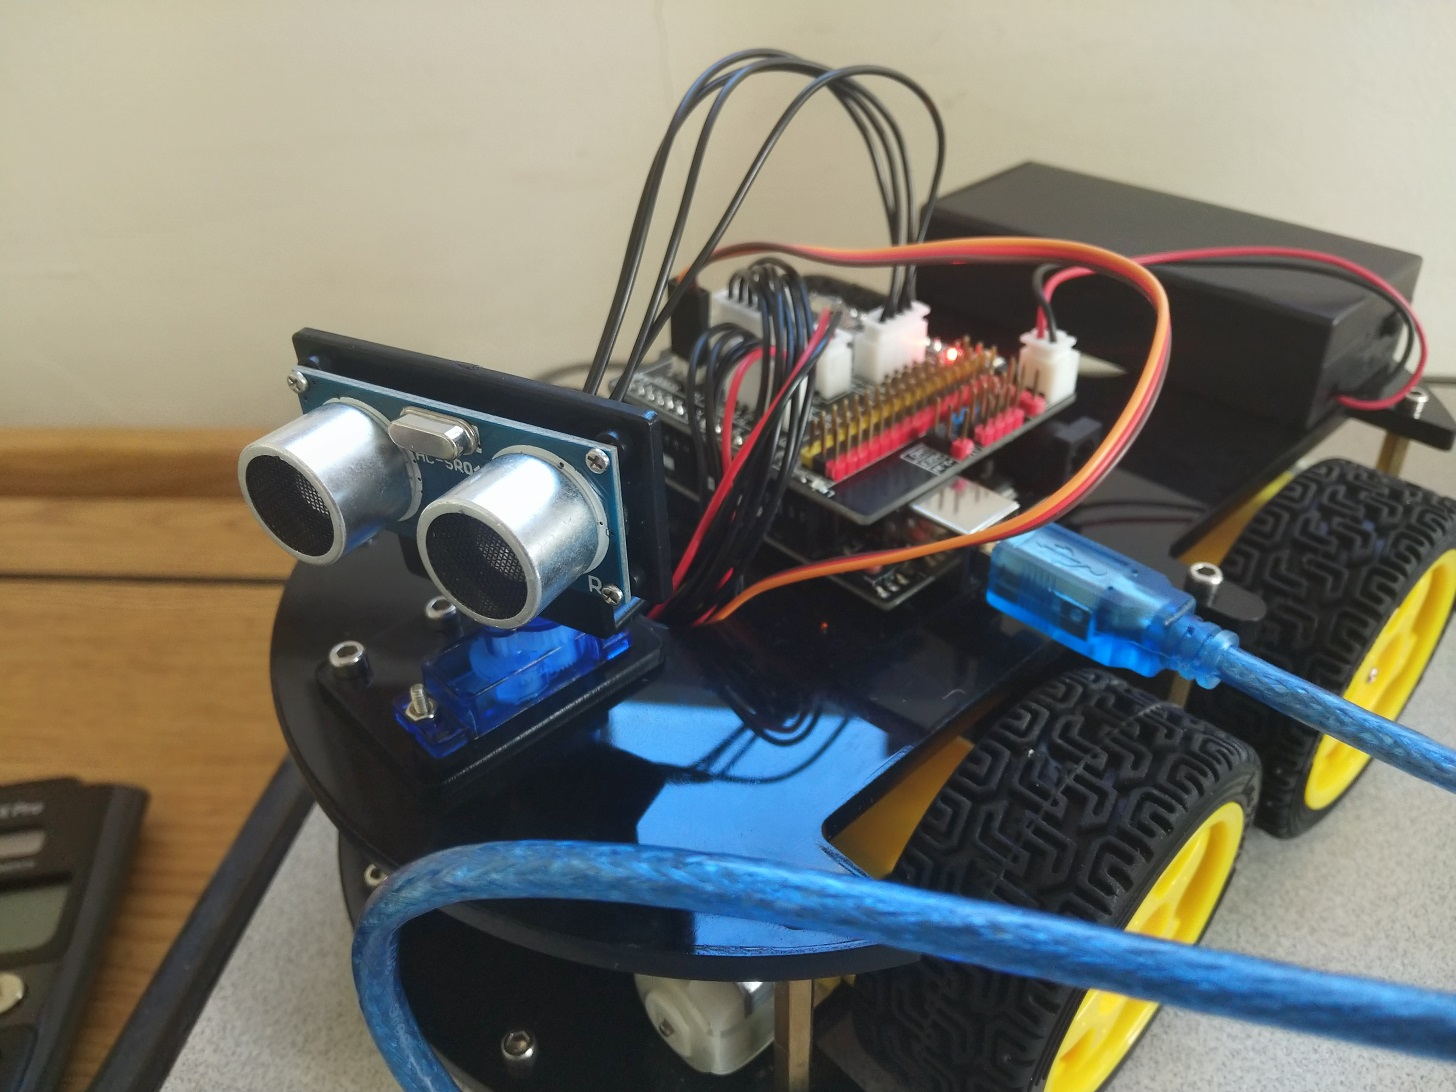
\includegraphics[width=\linewidth]{robot.jpg}
\end{center}
\caption{Servo with ultrasonic sensor assembly.}
\label{fig:f4}
\end{figure}

\section*{Implementation}
For this lab we are writing our own servo controller that should simply 
convert and assign the correct pwm mode for an approximate direction.

\subsection*{initServo}
Initializes timer 2 and sets the phase to the correct 50 Hz signal. 
Also sets any pins needed by the servo.

\subsection*{moveServo}
Takes in a degree angle, maps to a PWM value then assigns to the PWM 
pin controlling the servo.

\subsection*{mapAngle}
Takes in an angle and returns a mapped PWM value for the angle, exposed 
to allow us to read and debug.

\section*{Discussion}
Timers and motor drivers are finicky devices, especially on platforms with 
some degree of inaccuracy. By their inherent design DC motors are not entirely 
accurate but made to be fast and provide continuous drive. One of our first 
issues was in driving the motors and accounting for issues with the quality 
of the build, especially power distribution and toe, camber, and alignment of 
the wheels on their motors. Some degree of physical manipulation was performed 
but we ultimately took to software solutions to bias the wheels correctly by 
adjusting the PWM value written to the output compare registers.

Another issue was using the correct data type. On initial sketch we used integers, 
however, we later recalled that these are in fact 16 bit values being assigned to 
8 bit accurate registers. To prevent overflow, we changed these to 8 bit c-character 
variables immediately.

This lab is fairly straightfoward, using the OCR0X registers directly to write a 
relative speed between 0-255 in fast PWM mode on a 1024 prescale, we can more or 
less come to approximate to the easy mode Arduino IDE sketch of setting the digital 
pins PWM of 0-255. Then it's a matter of writing corresponding functions to 
make easier controlling the speed and direction to the motors.


\section*{Responses}
\begin{enumerate}
\item  PWM frequency for Timer 0 is controlled by the clock-select bits in TCCR0B. Test all five
PWM output frequencies while holding OCR0n static. What effects do you see on motor
speed/torque? Drawing on your knowledge from Circuits II, what is happening?

As we increase the prescaler, the motors start to whine to even higher pitches as we increase the scale
of the clock until what we suspect is a barely audible noise at 16MHz which is the absolute highest clock.
In addition, as we went up through the pre-scalers, there was a noticable loss of torque as the prescale value 
was increased. At a prescale value of 1, no prescale, we suspect there's some resolution or overflow happening, as 
the motors remained on full power as it ran through the lab test program.

The internal of the motor is a coil of wire around a magnet which is attempting to either attract itself 
or deflect itself against the poles of the magnet and the poles of the magnetic inductive force around the 
driving coils. When our prescale value is too high for this reaction to take place and affects the total duty
cycle available to the DC motor. In the case of the extremely high frequencies to our motors, the full duty 
cycle is not being executed.



\item  Watchdog timers are a critical part of robust embedded systems. How do watchdog timers
function? Does the ATMega328P include a watchdog timer? If so, from where does it pull
its clock signal? To what value would one set WDTCSR if they wanted to reset the system
after one second of inactivity?

A watchdog timer is a timer that, when hitting a timeout, will attempt to reset the entire 
system. This is generally used to check for faults or large values of other timers and systems 
to prevent hanging of the entire system. It's generally good practice to reset or refresh the watchdog 
timer value at the end of certain processes to ensure it doesn't erroneously reset the entire system.

The ATMega328P does have a watchdog timer which pulls from it's own independent clock generator. One 
would set the last four bits of the WDTCSR register to 0110 for a one second watchdog timer.


\end{enumerate} 

\newpage
\section*{Appendices}
Table of contents:
\begin{itemize}
    \item main.c - entry, initialization and drive instructions
    \item bit\_macros.h - bit manipulations macros
    \item motor\_driver.h - header file for main motor driver
    \item motor\_driver.c - main c file for motor driver
    \item pin\_map.h - map of our motor pins
\end{itemize}
\newpage

\section*{Appendix A: main.c}
\begin{tiny}
\lstinputlisting{../main.c}
\end{tiny}
\newpage

\section*{Appendix B: bit\_macros.h}
\begin{tiny}
\lstinputlisting{../bit_macros.h}
\end{tiny}
\newpage

\section*{Appendix C: motor\_driver.h}
\begin{tiny}
\lstinputlisting{../motor_driver.h}
\end{tiny}
\newpage

\section*{Appendix D: motor\_driver.c}
\begin{tiny}
\lstinputlisting{../motor_driver.c}
\end{tiny}
\newpage

\section*{Appendix E: pin\_map.h}
\begin{tiny}
\lstinputlisting{../pin_map.h}
\end{tiny}
\newpage

\end{document}
\grid
